
\documentclass{article}
\usepackage{subfigure}
\usepackage{amsmath}
\usepackage{float}
\usepackage{ragged2e}
\usepackage{amssymb}
\usepackage[utf8]{inputenc}
\usepackage{pmboxdraw}
\usepackage{graphicx} \graphicspath{
{./images/} }
\usepackage{indentfirst}
\usepackage{multicol}
\usepackage[a4paper, total={6.5in, 8.5in}]{geometry}
\DeclareSymbolFont{letters}{OML}{ztmcm}{m}{it}
\newtheorem{definition}{Definition}
\newtheorem{remark}{Remark}
\newtheorem{theorem}{Theorem}
\newtheorem{wrnote}{Writing note}
\newtheorem{proof}{Proof}

\title{\textbf{Modelling Neuroplasticity: Using Machine Learning to Learn About TMS Data}}
\author{Santiago López Pereyra, Jennifer Goldschmied, Coauthor 3,
Coauthor 4, \ldots}
\maketitle

\begin{document} 

\begin{multicols}{2}

\section{Introduction}

The emergence of new computational models has provided neuroscientists with
novel ways of extracting significant insights from experimental data. This paper
takes a computational approach to challenges arising from the analysis of
transcranial magnetic stimulation (TMS) data under the double pulse paradigm. We
argue that using indicators of neuroplasticity for each specific double
stimulation, as opposed to their average, allows for the use of data-driven
methods of analysis. 

Particularly, we formulate pulse-specific measures of relative amplitude between
paired and test pulses. These measures represent the proportionality of specific
paired-pulse responses with respect to test-pulse responses. Namely, they serve as
proxies for neuroplasticity in the brain by capturing the degree of
inhibition or facilitation induced by each double-stimulation.

The benefits of data-driven methods of analysis cannot be overstated. Their
potential implication in the production of scientific evidence and the
diagnosis of clinical disorders go beyond the scope of this paper and deserve
further investigation.


\section{Background}

Transcranial magnetic stimulation (TMS) is a common,
non-invasive experimental technique used to evoke action
potentials in cortical regions of the brain. In particular,
researchers often target the motor cortex and measure the
motor evoked potential (MEP) aroused by the stimulation.
When the purpose of the experiment is to inquire on
neuroplasticity, such stimulations are performed under the
\textit{paired pulse paradigm}.

The \textit{paired pulse paradigm} (or \textit{double pulse
paradigm}) consists in eliciting a series of two temporally
proximate pulses (in the order of miliseconds). The evoked
potentials of the double-stimulation are compared to those
of single test stimulations, and their relative amplitude is
taken as a proxy of neuroplasticity in the brain. The time
separating each of the paired pulses is termed
\textit{interstimulus interval} (ISI). It is the general
case that low intervals (4 or 5 miliseconds) produce
intracortical inhibition, with the evoked potentials of
paired stimulations being generally lower than those of
single pulses. Greater intervals, on the other hand, tend to
produce facilitation. 


In the context of this paper, we shall term any coefficient that serves to
represent the proportional relationship between the potentials evoked by paired
and test pulses a \textit{measure of relative amplitude} (MRA).

The goal of this paper is to provide pulse-specific measures of relative
amplitude. This is, coefficients that represent the relative amplitude of each
individual paired pulse with respect to the set of test pulses in an
experimental session. The benefit of this is that it keeps data resolution at
its highest, which allows for the implementation of data-driven artificial
intelligence in the analysis of the experimental results. Thus, from a computer
science perspective, our objective is constrained to the sphere of feature
engineering. 

We will show how pulse-specific measures of relative amplitude allow for
otherwise unfeasible computational analyses of TMS data, such as the use of
machine learning models for the detection of different pulse-response patterns
among different groups of clinical subjects. In particular, we will show they
allow for a machine learning classifier to correctly determine whether a
subject belongs to one of four clinical categories, based only on its evoked
potentials and across different inter-stimulus intervals, with an accuracy of up to
$90\%$.

\section{Dataset}

Our case study uses data from $N = 43$ subjects at UPenn's \textit{Lab for the
Study of Slow-wave sleep activity}, with $H = 17$ healthy controls (HC) and $D =
26$ with major depressive disorder (MDD). Subjects received transcranial
magnetic stimulation of the motor cortex after both a night of baseline sleep
and a night of slow-wave disruption (SWD) sleep. The stimulations were performed
under the double pulse paradigm. Per session, subjects received twenty-four
($24$) test pulses in total and eight ($8$) paired pulses per ISI. The ISIs were
$4, 5, 8, 10, 15$ and $20$. The evoked potentials were measured by placing an
EMG electrode on the targeted muscle of the thumb. In the slow-wave disruption
session, we sent a constant auditory stimulus with sufficient strength to
interrupt the normal occurrence of slow-wave sleep, yet not strong enough to
wake the subjects.

Please see the table below to see the resulting subject categories:

~

~

\begin{tabular}{ |p{2cm}|p{2cm}|p{2cm}|  }
\hline
& Baseline & Slow-wave disruption \\
\hline
Healthy control & HC BL & HC SWD \\
\hline
Major depressive disorder & MDD BL & MDD SWD \\
\hline
\end{tabular}

~

~

Each observation comes from an individual transcranial stimulation. The features
of the resulting database are:

\begin{enumerate}
    \item An $EMG$ variable with the peak-to-peak EMG of each elicited pulse.
    \item A $Label$ categorical feature, which represents the group of
        the subject of each observation. 
    \item An $ISI$ feature that represents the inter-stimulus interval of each
        pulse. A value of $-1$ indicated that the given pulse was a test pulse (no
        inter-stimulus interval).
\end{enumerate}

The distribution of the evoked potentials is always exponential. However, the
$\beta$ parameter of the distribution varies across subject groups and session
types, as shown in Figures \ref{fig:figure1} and \ref{fig:figure2} and in the
table below:

~

    \begin{tabular}{ |p{2cm}|p{2cm}|p{2cm}|  }
    \hline
    &       Mean & Median \\
    \hline
    HC BL & 196.77 & 149.36 \\
    \hline
    HC SWD & 165.98 & 99.76 \\
    \hline 
    MDD BL & 187.56 & 127.69\\ 
    \hline 
    MDD SWD & 247.57 & 151.07 \\
    \hline
    \end{tabular}

~ 

Observe that each of the means in the above table corresponds to the estimated
$\beta$ parameter of the distribution of the paired pulses on each subject
group.

\begin{figure*}
  \begin{minipage}[b]{0.48\linewidth}
    \centering
    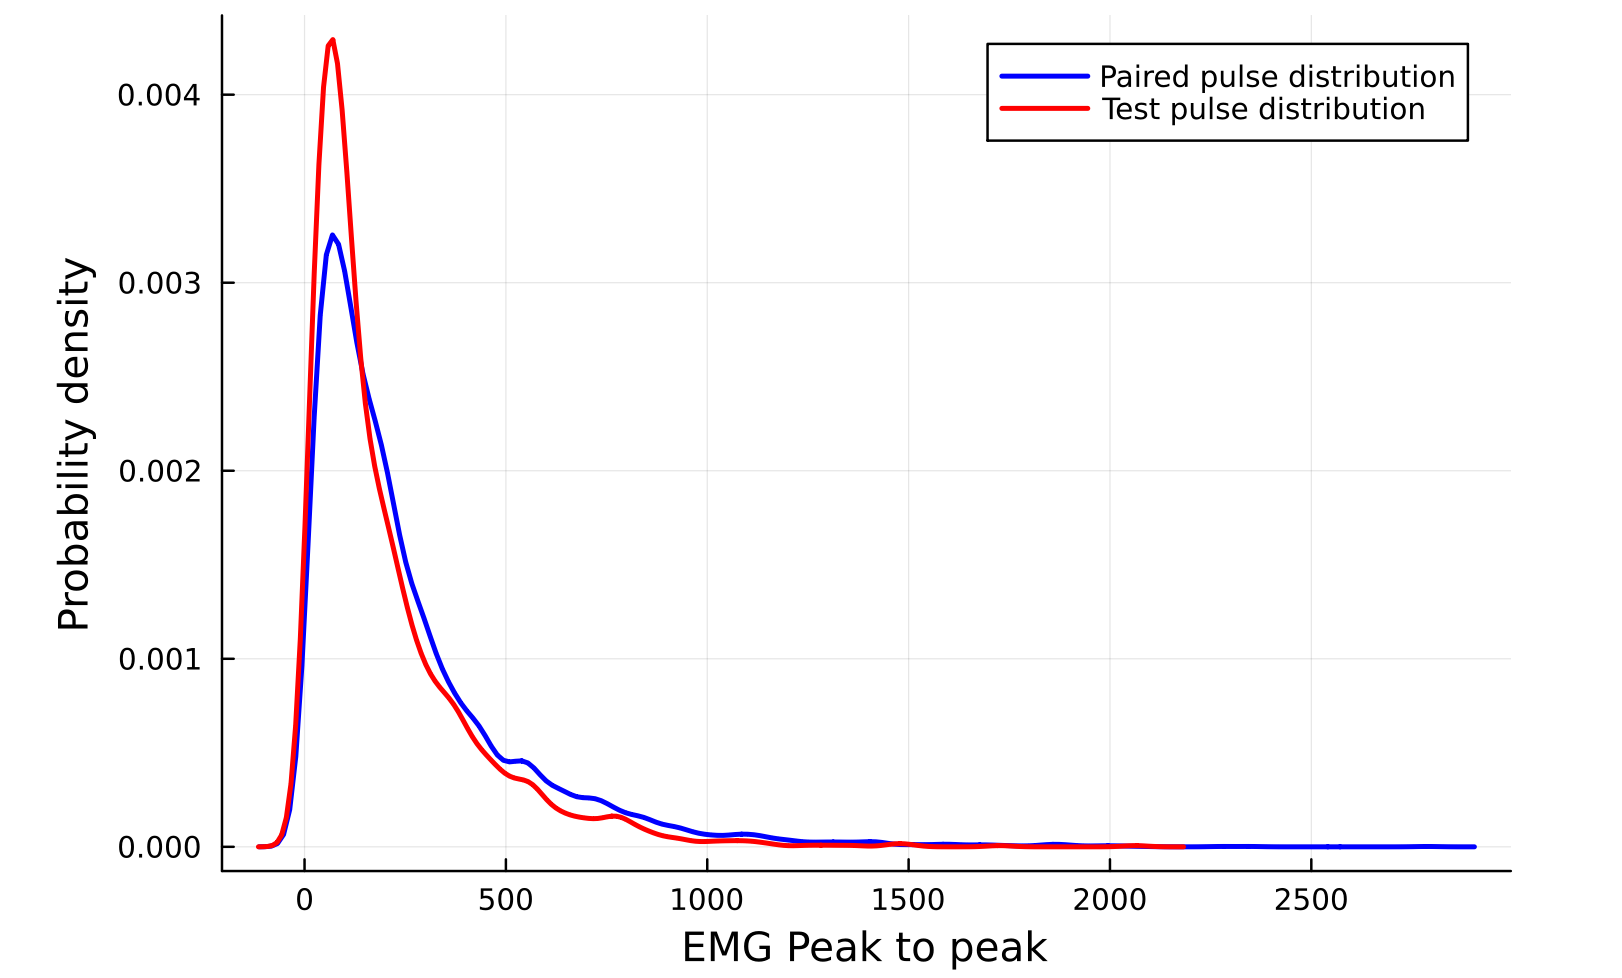
\includegraphics[width=\linewidth]{Paired-TestDist}
    \caption{Distribution of paired and test pulses}
    \label{fig:figure1}
  \end{minipage}
  \hspace{0.04\linewidth}
  \begin{minipage}[b]{0.48\linewidth}
    \centering
    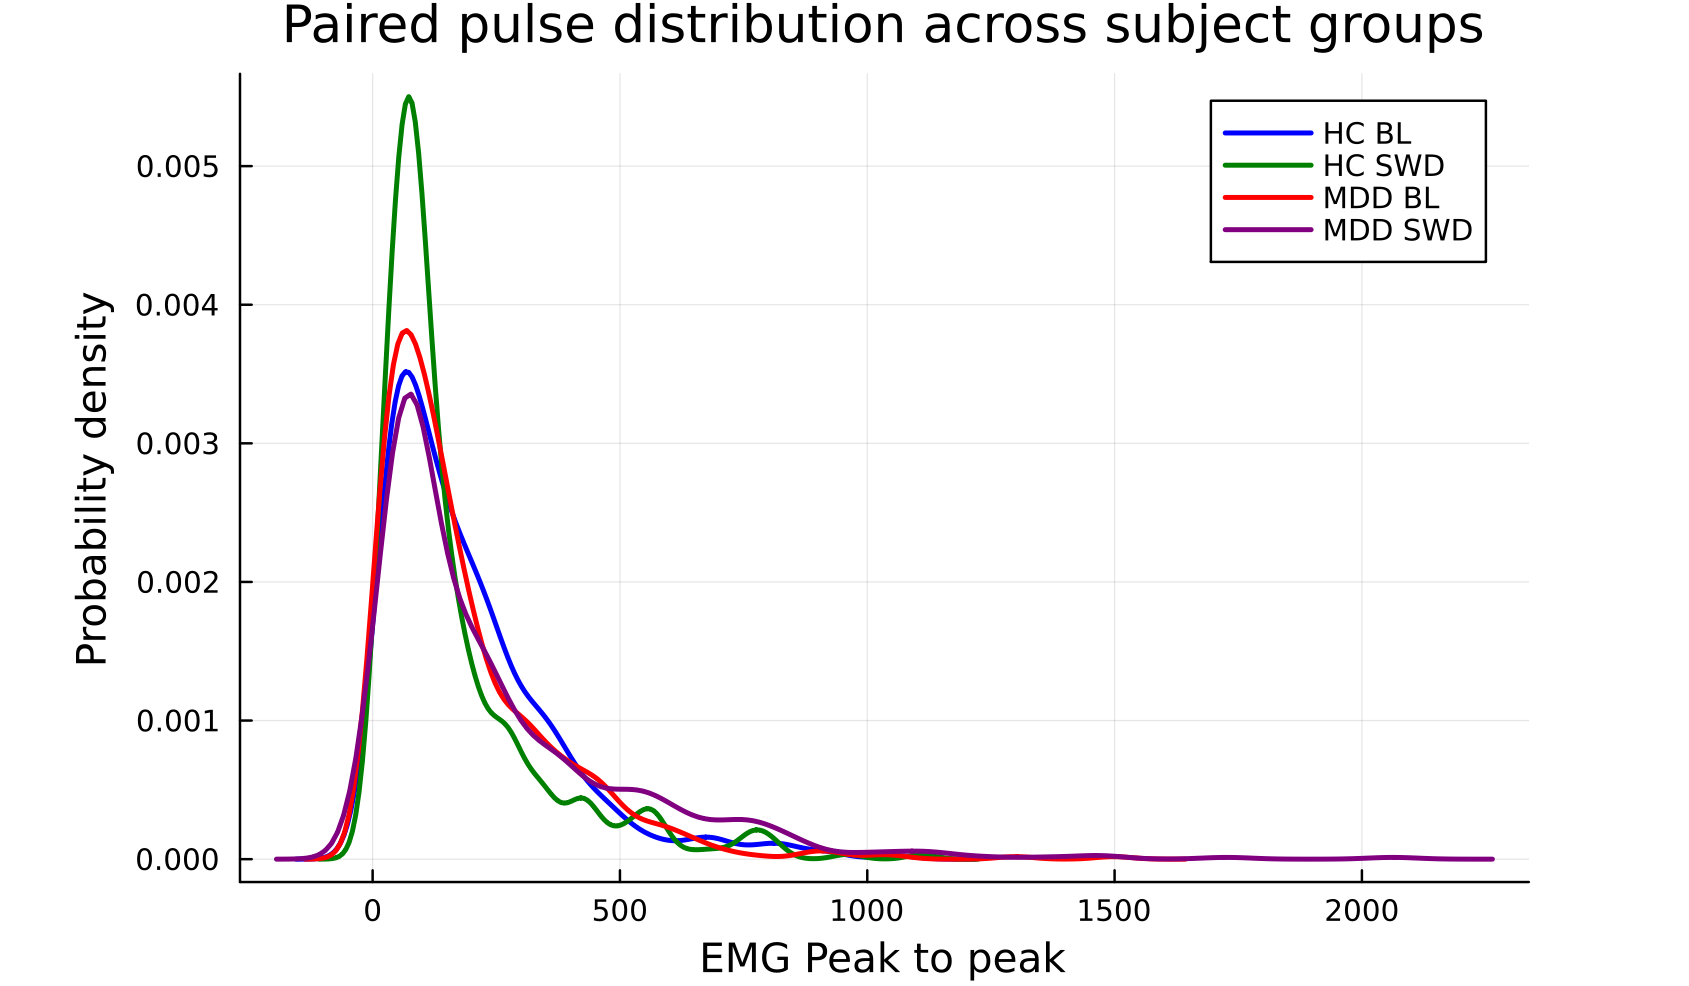
\includegraphics[width=\linewidth]{P-dist-subjects-big}
    \caption{Distribution of paired pulses across subject groups}
    \label{fig:figure2}
  \end{minipage}
\end{figure*}



\section{Limitations of the traditional TMS method of analysis}


Measures of relative amplitude in neuroscience are generally computed at the
subject and group level by repeatedly taking averages. This is natural, since
scientific interest generally resides in evaluating differences across subject
groups. However, it also raises problems pertaining to
the downscaling of the data resolution and the reliability of the resulting values.

The procedure to establish the average relative amplitude of a group of subjects
(for example, healthy controls) is simple. Traditionally, it involves taking the
quotient of the average paired-pulse and the average test pulse responses per
every subject. Next, those quotients are averaged out across all subjects in the
subject group. In short, it is an average of averages. 

Although this practice is not arbitrary ---since hypotheses generally deal with differences
across subject groups--- it has three major limitations. Firstly, it implies
greatly downscaling the data resolution, making data-driven methods of analysis
unfeasible. Secondly, potentials evoked by test and paired pulses present a very
high variance (Rossini et. al., 20015; Orth, Snijders and Rothwell, 2003;
Wassermann, 2002), which —being that it is a quotient of two means—  raises
questions about the quality of the representation where relatively few pulses
are elicited. Thirdly, our observations suggest potentials evoked by TMS
stimulations follow an exponential distribution, which puts in question whether
arithmetic means are a reliable measure of central tendency.

To make matters worse, when considering the size of the data across multiple
experimental subjects, the shrinkage in data resolution is far from negligible.
And in times when scientific inquiry can greatly benefit from forms of
artificial intelligence that rely on large amounts of data (e.g. machine
learning), it is clearly limiting to count solely with low-resolution measures
to interpret experimental results.


\section{Proposed approach}

\subsection{Pulse-specific relative amplitude measures}

In light of the technical concerns about the traditional approach, this paper
proposes two pulse-specific relative amplitude measures. This allows for
otherwise unfeasible computational analyses of TMS data, such as the use of
machine learning (ML) models for the detection of different pulse-response
patterns among different groups of clinical subjects.

Pulse-specific measures of relative amplitude are coefficients that represent,
for every experimental subject, the proportionality of each individual
paired-pulse response with respect to the set of \textit{all} test-pulse
responses. From a neuroscientific perspective, they are a proxy for
neuroplasticity at the level of each particular stimulation, measuring the
amount facilitation or inhibition in each specific response. From a
computational perspective, these measures prescind from the need of averaging
paired-pulses out, and thus keep data resolution at its highest.

In order to test these measures, we look at whether they improve the performance
of a ML classification model and in what degree.\footnote{We use a
classification model for practical reasons ---namely, because the samples in our
data were conveniently labeled by subject group and sleep session.} Our case
study is a random forest model in Python tasked with classifying every
observation with the appropriate subject label. The model we use is an AdaBoost
classifier consisting of 20 decision trees. Every tree in the ensemble has a
maximum depth of $8$. The boosting algorithm is \textit{SAMME.R}. The learning
rate is set to $\eta = 0.01$. We use holdout cross-validation to evaluate the
performance of the model. The total number of values in our dataset is $n =
9382$.

The goal of the classifier is to infer, based on the properties of each TMS
response, the group of the subject upon which the stimulation was elicited, as
well as the type of sleep session after which it occurred. Our hypothesis is
that pulse-specific measures of relative amplitude will significantly improve
the model's performance.


Section \textbf{5} provides the mathematical definitions of our measures of
relative amplitude. Section \textbf{6} discusses the impact of each measure on
the performance of the random forest model. Specifically, section \textbf{6.1}
shows the performance of the model when trained over the raw data (i.e. the
features described in section \textbf{3.1}). Section \textbf{6.2} shows the
performance of the model when including pulse-specific measures of relative
amplitude. Section \textbf{6.3} shows the performance of the model when combining the
pulse-specific measures with logarithmic transformations of the raw data and the
use of weighted instead of arithmetic averages.

As for the computation of these measures, we implemented the formulas of section
\textbf{5.2} for every TMS response using the Julia programming language.



\subsection{Definitions: Pulse specific relative amplitudes}

For simplicity, we will first deal with the hypothetical situation in which a
single ISI is used for paired stimulations in a unique TMS session. Our
formulations generalize easily to different inter-stimulus intervals and
multiple experimental sessions.

Firstly, we need to establish some convenient notation. Let $n$ and $m$ be the
number of paired and test pulses elicited to the subject in the session,
respectively. Let $\textbf{x}$, $\textbf{t}$ be vectors over the $\mathbb{R}^+$
vector space whose components are understood to be the evoked potentials of
paired and test stimulations, respectively.


\begin{definition} 


    Let $x \in \textbf{x}$ be the evoked potential of a single paired
    stimulation. Then we define two pulse-specific relative amplitude measures,
    $\rho : \mathbb{R} \to \mathbb{R}, \delta : \mathbb{R} \to \mathbb{R}$,
    where

    \begin{equation} 
        \rho(x) := \frac{mx}{\sum_{i=1}^mt_j}
    \end{equation}

    \begin{equation} 
        \delta(x) := \frac{x}{m}\sum_{j=1}^m\frac{1}{t_j} 
    \end{equation}
\end{definition}

\begin{theorem} 
    $\forall x: x \in \mathbb{R}^+:\delta(x) \geq \rho(x)$. (For a proof of this
    property, consult the appendix.) 
\end{theorem}

Notice that $\rho(x)$ is the proportion between the potential $x$, evoked by a
paired stimulation, with respect to the average potential of single test
stimulations. On the other hand, $\delta(x)$ is the average proportion of $x$
with respect to each single test pulse. 

To put it differently, $\rho$ is a representation of the relative importance of
each double pulse in relation to the overall distribution of the test pulses in
the subject. It measures the deviation of the double pulse $x$ with respect to
the average test pulse. $\delta$, in contrast, measures the proportionality of a
double pulse with respect to different values in the distribution of the test
pulses of the subject.

Notice as well that $\rho$ and $\delta$ are defined over the evoked potentials
of a specific experimental session. In other words, whenever we speak of the
$\delta$ and $\rho$ \textit{features} (\textit{id est}, of the data resulting
from broadcasting $\rho$ and $\delta$ over a collection of evoked potentials),
such features are understood to be subject- and session-specific.

\begin{theorem}
    Let $\pi$ denote the coefficient traditionally used for estimating the
    relative amplitude between test and paired pulses. In accordance to what was
    described in the second paragraph of Section $4$,

    \begin{align*}
        \pi = \frac{\mu_x}{\mu_t}
    .\end{align*}

    where $\mu_x, \mu_t$ are the mean paired and test pulse responses,
    respectively. It follows from the definition of $\pi$ and $\rho$ that

    \begin{align*}
        \pi = \frac{\rho(x_1) + \ldots + \rho(x_n)}{n}
    .\end{align*}

    (For a proof, consult the appendix.)
\end{theorem}

The second remark is of great importance. It states that the way in which
relative amplitude was traditionally computed---the way in which neuroplasticity
was traditionally proxied---is different from our proposed $\rho$ function only
in terms of scale. More specifically, the traditional coefficient used to proxy
neuroplasticity at the subject level is nothing but the mean $\rho$
measure in an experimental session. We believe this bestows $\rho$ with a
certain degree of confidence, insofar as not only it is not entirely new, but
neuroscientists have implicitly used it all along.


\subsection{Generalizing to multiple subjects}


\begin{definition}
    Let $\textbf{x} \in \mathbb{R}^j$ with $j \in \mathbb{N}$. Then $T:
    \mathbb{R}^j \to \mathbb{R}^j, R : \mathbb{R}^j \to \mathbb{R}^j$ are the
    linear transformations defined as

    $T(\textbf{x}) := \begin{bmatrix} 
        \rho(x_1) & \ldots & \rho(x_j)
    \end{bmatrix}^\intercal $ and $R(\textbf{x}) := \begin{bmatrix} 
        \delta(x_1) & \ldots & \delta(x_j) 
    \end{bmatrix}^\intercal $.
\end{definition}

It is trivial to show that $T$ and $R$ are linear mappings (consult the
Appendix). Now let $k \in \mathbb{N}$ denote the number of experimental subjects
in an experiment, to each of whom $n, m$ paired and test pulses were elicited,
respectively.

\begin{definition}
    We define $\textbf{P} \in \mathbb{R}^{k \times n}$ a
    matrix where the $i$th row vector $\textbf{x}^{(i)}$ is the vector whose
    components are the paired-pulse responses of the $i$th subject.
\end{definition}

\begin{definition}
    Let $\mu^{(t)}_i$ be average test-pulse response of the $i$th subject. Let
    $\mu^{(t)^{-1}}_i$ be the average \textit{reciprocal} test-pulse response of
    the $i$th subject. Then $\textbf{M}^{k \times k}$ is a diagonal matrix with
    $\textbf{M}_{(ii)} := \frac{1}{\mu^{(t)}_{i}}$, and $\textbf{M'}^{~ k \times
    k}$ is a diagonal matrix with $\textbf{M'}_{ii} := \mu^{(t^{-1})}_i$.
\end{definition}

\begin{theorem}
    The row-vectors of $\textbf{X}_\rho = \textbf{M}\textbf{P}$ are the
    vectors $T(\textbf{x}^{(1)}), \ldots, T(\textbf{x}^{(k)})$, and
    the row-vectors of $\textbf{X}_\delta = \textbf{M'}\textbf{P}$ 
    are the vectors $R(\textbf{x}^{(1)}), \ldots,
    R(\textbf{x}^{(k)})$.
\end{theorem}


If experiments were conducted using multiple ISI, then to each ISI $r$ it
corresponds a distinct matrix $\textbf{X}_\delta^{ISI = r},
\textbf{X}_\rho^{ISI = r}$. The same applies to different subject groups.

We have expanded $\rho, \delta$ to higher dimensions for the purpose of
providing a theoretical framework of their application to larger data sets and
many experimental subjects. However, it is important to note that the matrix
representations here presented only make sense under the assumption that, on
each subject, none of $n$ paired pulses were anomalous, and hence all can be
safely included in the model. Such assumption rarely holds in reality, where it
is usual to excluded some pulses due to the presence of artifacts. There are
many ways to deal with this situation in the implementation of our model---the
safest being the direct application of $T$ and $R$ to the data vectors---. Thus,
more than serving the algorithmic implementation of the model, which may
prescind from them, these matrices provide insight into the exact nature of the
transformations involved in the model.


\section{Results}

\subsection{Random forest without MRA}

The first random forest model is our control group. We trained it on the raw
data ---that is, without the inclusion of pulse-specific MRA. The model's
accuracy on the testing set was of $\approx34.2 \%$. The confusion matrix of the
model, \textbf{Figure 3.}\textit{a}, shows that errors concentrated towards
healthy control categories. Additionally, the categorization of diagnosed
subjects was poor, although substantially better than that of healthy controls. 

Although the model almost never confuses an MDD subject with a healthy control,
this does not necessarily imply that the model is capturing key differences
between these groups. On the contrary, this is more likely a consequence of the
model's bias in favour of the MDD categories. This bias is probably caused by
the fact that the dataset has more MDD subjects than healthy controls. In
consequence, the model learns the rudimentary strategy of always guessing for
one of the MDD categories.

\subsection{Random forest with MRA}

The following models incorporated the $\rho$ feature, then the $\delta$ feature,
and then both, respectively. The inclusion of the $\rho$ feature increased
accuracy by a factor of $\approx 2.1$ to $72.6\%$. Subsequently, the inclusion
of the $\delta$ feature had a similar impact, increasing accuracy to $73.4\%$.
Lastly, the inclusion of both the $\delta$ and $\rho$ features improved accuracy
to $\approx 87.1\%$. The confusion matrix of the model trained with both $\rho$
and $\delta$ can be observed in \textbf{Figure 3.}\textit{b}.

\begin{figure}[H]
  \centering
  \subfigure[Raw data]{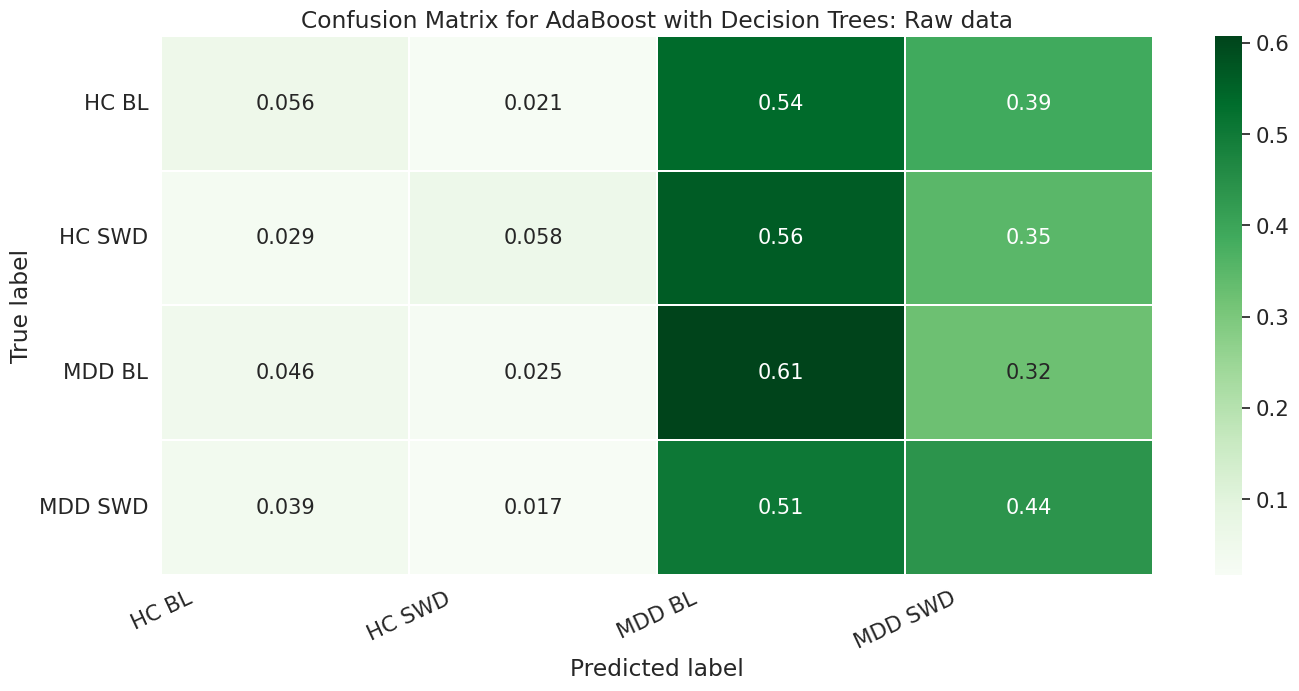
\includegraphics[width=0.48\textwidth]{cm-raw}}
  \hfill
  \subfigure[$\rho$ and $\delta$ features included.]{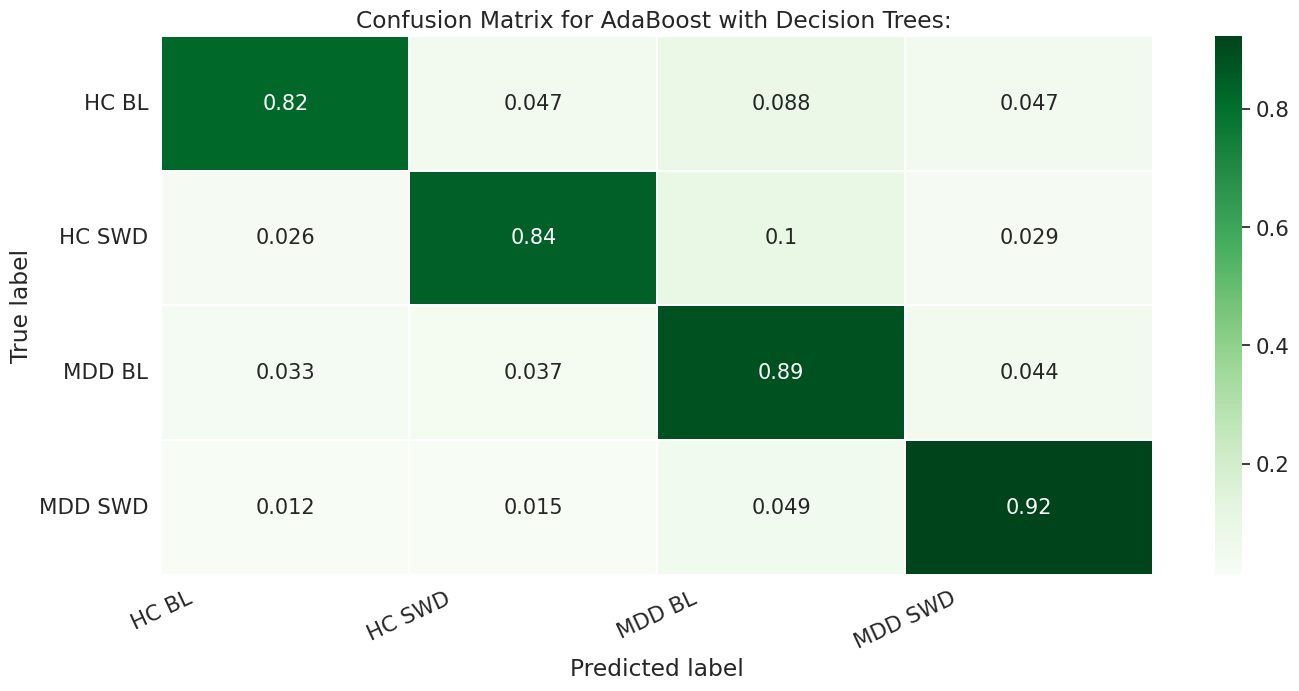
\includegraphics[width=0.48\textwidth]{cm-rho-delta}}
  \caption{Compared performance: raw data and data with measures of relative
  amplitude.}
  \label{fig:two_images}
\end{figure}


\subsection{Random forest with additional features}

Since the neural response to transcranial stimulations follows an exponential
distribution (see Figures 1 and 2), we tested the $\rho$ and $\delta$ functions
over the logarithmically transformed peak-to-peak EMG. This had a negligible
positive impact in the overall performance.

On the contrary, the inclusion of weighted variants of the features defined
above greatly improves the performance of the model. The use of weighted instead
of arithmetic averages in the formulas for $\delta$ and $\rho$ is useful in
dealing with the excessive influence of outliers or highly spread out points in
the feature. For example, the weight vectors may be computed using the MAD or
the inverse-variance of each $t \in \textbf{t}$. 

For example, using inverse-variance weights accuracy increased to $\approx
90.2\%$. The confusion matrix of this last model can be appreciated in
\textbf{Figure 4}.

\begin{figure}[H]
    \centering
    \subfigure[$\rho, \delta, \rho(\ln x), \delta(\ln x), \rho_w$ and $\delta_w$
    included.]{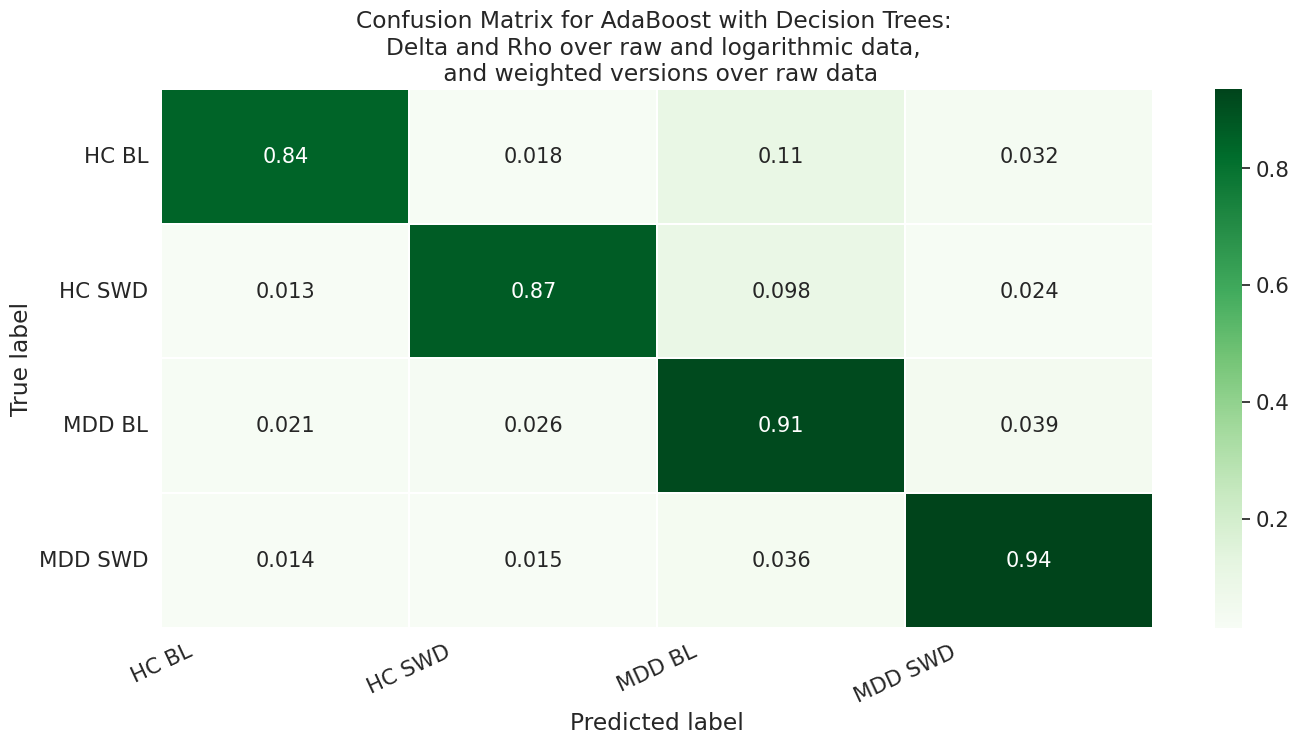
\includegraphics[width=0.48\textwidth]{final-cm}}
    \caption{Confusion matrix}
    \label{fig:figure4}
\end{figure}

In summary, our results demonstrate that pulse-specific MRA greatly improve the
accuracy of a random forest model trained over TMS data for subject
classification. More importantly, it becomes clear that, by using the engineered
features $\delta$ and $\rho$, researchers can attain evidence in favour or
against hypotheses pertaining to differences among subject groups. Particularly,
the model provides otherwise unattainable evidence in favour of sleep-modulated,
depression-induced differences in neuroplasticity.

\section{Conclusion}

This paper shows that pulse-specific relative amplitude measures allow for the
use of machine learning models over TMS experimental data. Such models
can play an important part in TMS research by introducing new ways of
both analyzing and extracting meaningful insights from the experimental results.

The use of machine learning models in neuroscientific observations is not only a
promising tool in the production of evidence. There is a diagnostic potential
that is yet to be evaluated. By detecting distinct neural patterns between
healthy control and diagnosed subjects,\footnote{At least under specific
experimental conditions.} these models can potentially serve as a useful tool in
the diagnostic process.

Although long and serious scientific effort is still required to appraise the
diagnostic potential of these technologies, we believe our results allow
for cautious optimism on the matter.

It should however be noted that, although machine learning models reveal
distinct response patterns and differences across subjects, they do not disclose
the neurobiology modulating those differences nor what those patterns are. 

Lastly, the impact of pulse-specific MRA in data-driven models other than random forests
is yet to be tested. These empirical trials are not trivial because failure or
success of the models is dependent not only on the engineered features, but on
the nature of the experimental data itself. 

\end{multicols}

\section{References}

\begin{enumerate}
    \item Lefaucheur, JP. “Transcranial Magnetic Stimulation.” Handbook of clinical neurology. U.S. National Library of Medicine. Accessed April 14, 2023. https://pubmed.ncbi.nlm.nih.gov/31277876. 
    \item Orth, M, AH Snijders, and JC Rothwell. “The Variability of Intracortical Inhibition and Facilitation.” Clinical neurophysiology : official journal of the International Federation of Clinical Neurophysiology. U.S. National Library of Medicine. Accessed April 14, 2023. https://pubmed.ncbi.nlm.nih.gov/14652096/. 
    \item Rossini, PM, D Burke, LG Cohen, Z Daskalakis, R Di Iorio, V Di Lazzaro, F Ferreri, et al. “Non-Invasive Electrical and Magnetic Stimulation of the Brain, Spinal Cord, Roots and Peripheral Nerves: Basic Principles and Procedures for Routine Clinical and Research Application. an Updated Report from an I.F.C.N. Committee.” Clinical neurophysiology : official journal of the International Federation of Clinical Neurophysiology. U.S. National Library of Medicine. Accessed April 14, 2023. https://pubmed.ncbi.nlm.nih.gov/25797650/. 
        \item Wassermann, EM. “Variation in the Response to Transcranial
            Magnetic Brain Stimulation in the General Population.” Clinical
            neurophysiology : official journal of the International Federation
            of Clinical Neurophysiology. U.S. National Library of Medicine.
            Accessed April 14, 2023. \newline https://pubmed.ncbi.nlm.nih.gov/12088713/. 
\end{enumerate}

\pagebreak

\begin{multicols}{2}

\section{Appendix}

\textbf{Proof 1}. In \textbf{Remark 1}, we observed the following property:

    \begin{align*}
        \forall x: x \in \mathbb{R}^+ : \delta(x) \geq \rho(x)
    .\end{align*}

Such property can be proven via induction. Firstly, recall that


\begin{align*} \delta(x) &= \frac{x}{m}\sum^m\frac{1}{t_j} \\
                \rho(x) &= \frac{xm}{\sum^m t_j} \end{align*}


Let $S_1^m = \sum^m\frac{1}{t_j}, S_2^m= \sum^m t_j$. We operate under the
assumption that $t_i \in \mathbb{R}^+$. It is the case that

\begin{align*} 
    \frac{x}{m}\sum^m\frac{1}{t_j} &\geq \frac{xm}{\sum^m t_j} \\ 
    S_2^mS_1^m &\geq m^2
\end{align*}

This holds for $m=1$, since $\frac{1}{t_1}+t_1 \geq 1 \iff 1+t_1^2 \geq t_1$. So
we may assume $S^k_1 S^k_2 \geq k^2$ . We now set out to show that

\begin{equation*} 
    S^{k+1}_1 S^{k+1}_2 \geq (k+1)^2
\end{equation*}

This can be proven as follows.

\begin{align*} 
    S^{k+1}_1 S^{k+1}_2 &\geq (k+1)^2 \\ 
    (S_1^k+\frac{1}{t_{t+1}})(S_2^k+t_{k+1}) &\geq k^2+2k+1 \\
    S^k_1S^k_2+ t_{k+1}S_1^k + \frac{1}{t_{k+1}}S^k_2+1 &\geq k^2+2k+1 \\
    S^k_1S^k_2+ t_{k+1}S_1^k + \frac{1}{t_{k+1}}S^k_2 &\geq k^2+2k 
\end{align*}

We know $S^k_1S^k_2 \geq k^2$ and then it suffices to show $t_{k+1}S_1^k +
\frac{S^k_2}{t_{k+1}}\geq 2k$. To prove this, simply observe that

\begin{align*}
    \frac{1}{t_{k+1}}\sum_{j=1}^mt_j+t_{k+1}\sum_{j=1}^m\frac{1}{t_{j}} &\geq 2k \\
    \Big(\frac{t_1}{t_{k+1}}+...+\frac{t_k}{t_{k+1}}\Big)+\Big(\frac{t_{k+1}}{t_1}+...+\frac{t_{k+1}}{t_k}\Big)
    &\geq 2k \\ \iff
    \overbrace{a+\frac{1}{a}+b+\frac{1}{b}+... +
    n+\frac{1}{n}}^{\text{$2k$ terms} } &\geq 2k
\end{align*}

We have $\min f=2$  for $f(x)=x+\frac{1}{x}$ for $x \in \mathbb{R}^+$. Then
$\min(a+\frac{1}{a}+...+n+\frac{1}{n})=2k$ for $a,..., n \in \mathbb{R}^+$,
which concludes the demonstration.

\textbf{Proof 2.} In \textbf{Remark 2}, we observe that $\rho$ is implicitly
used in the traditional measures of relative amplitude. Recall that such methods
consist in taking the average paired-pulse response and dividing it by the
average test-pulse response. It is easily observed that

\begin{align*} \frac{\mu_x}{\mu_d} = \frac{\frac{1}{n}\sum_{j=1}^n
        x_{j}}{\frac{1}{m}\sum_{j = 1}^m t_j} 
        = \frac{\rho(x_{1i})+\cdots + \rho(x_{ni})}{n}
\end{align*}

\begin{proof}[Theorem 1]

    Let $\sigma = \sum_{i=1}^m t_j$ and $c \in \mathbb{R}$. It follows directly
    from the definition of $\rho$ that

    \begin{align*}
        T(c\textbf{x} + \textbf{y}) &= \begin{bmatrix} \frac{m(cx_1) + y_1}{\sigma} &
        \ldots& \frac{m(cx_n + y_n)}{\sigma} \end{bmatrix}^\intercal \\ 
                                    &=\begin{bmatrix} 
                                        \frac{mcx_1}{\sigma} +
                                        \frac{my_1}{\sigma} & \ldots &
                                        \frac{mcx_n}{\sigma} + \frac{y_n}{\sigma} 
                                    \end{bmatrix} \\
                                    &=cT(\textbf{x}) + T(\textbf{y})
    \end{align*}

    The proof the $R$ is linear is practically identical.
\end{proof}

\end{document}

